

\section{Motivation and Background}

\subsection{Large Language Models (LLM)}
Natural language processing (NLP) has always been an intricate field because of the complexity of how humans communicate.
It is challenging for a computer to replicate or learn text communication and expressions. However, this changed with the introduction
of Large Language Models (LLM) \textbf{[REFERENCE]}. These models are trained with large amounts of data to replicate human-like patterns,
and all was made possible because of transformers. This architecture differs from others because it uses self-attention \textbf{[REFERENCE]} \ref{transformer}.
This self-attention finds dependencies between all words in a text, short and long-term. In other words, it combines all possible 
positions of words within a text and assigns them a vector value. This enables the model to understand the meaning of words within a sentence. 

\begin{figure}[!htb]
    \centering
        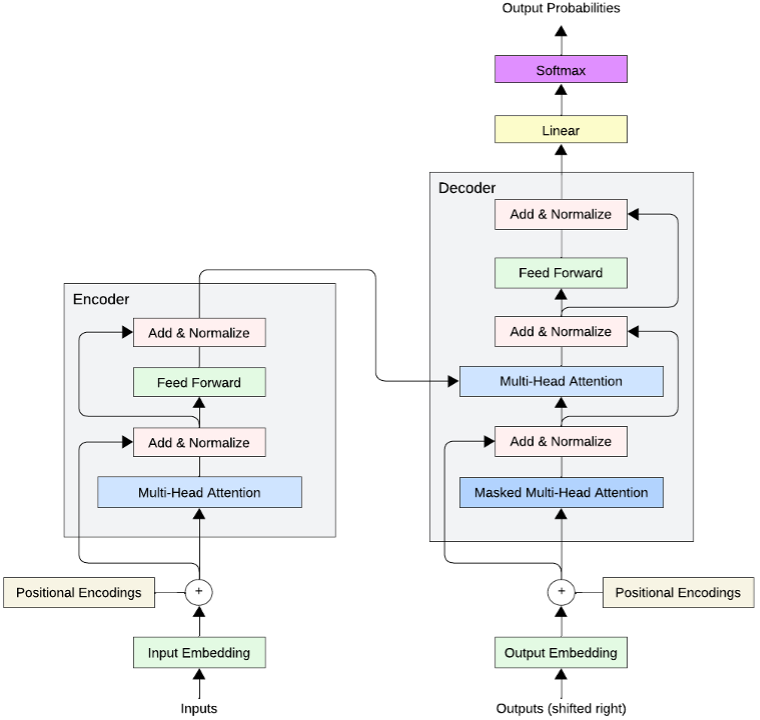
\includegraphics[width=0.75\linewidth]{figures/transformers_architecture.png}
        \caption{The transformer architecture}
        \label{transformer}
\end{figure}



The are three different architectures for Large Language Models, encoder-only, decoder-only, and encoder-decoder. Each one has advantages on specific tasks. In Figure \ref{architecture}

\subsubsection{Encoder-only models}
These models are like BERT.
This type of model predict by masking specific words in a sentence.
The are better for classification and sentiment analysis.

\subsubsection{Decoder-only models}
For these model we have the well known GPT-3, Mistral, and LLaMa.
They receive one input and try to predict the entire text.
They are good for summarizing and text-generation.

\subsubsection{Encoder-Decoder models}
The encoder-decoder models are T5.
They mask entire sequences of text.
Good for translation and question and answering. \cite{9906925}

\begin{figure*}[!htb]
    \centering
        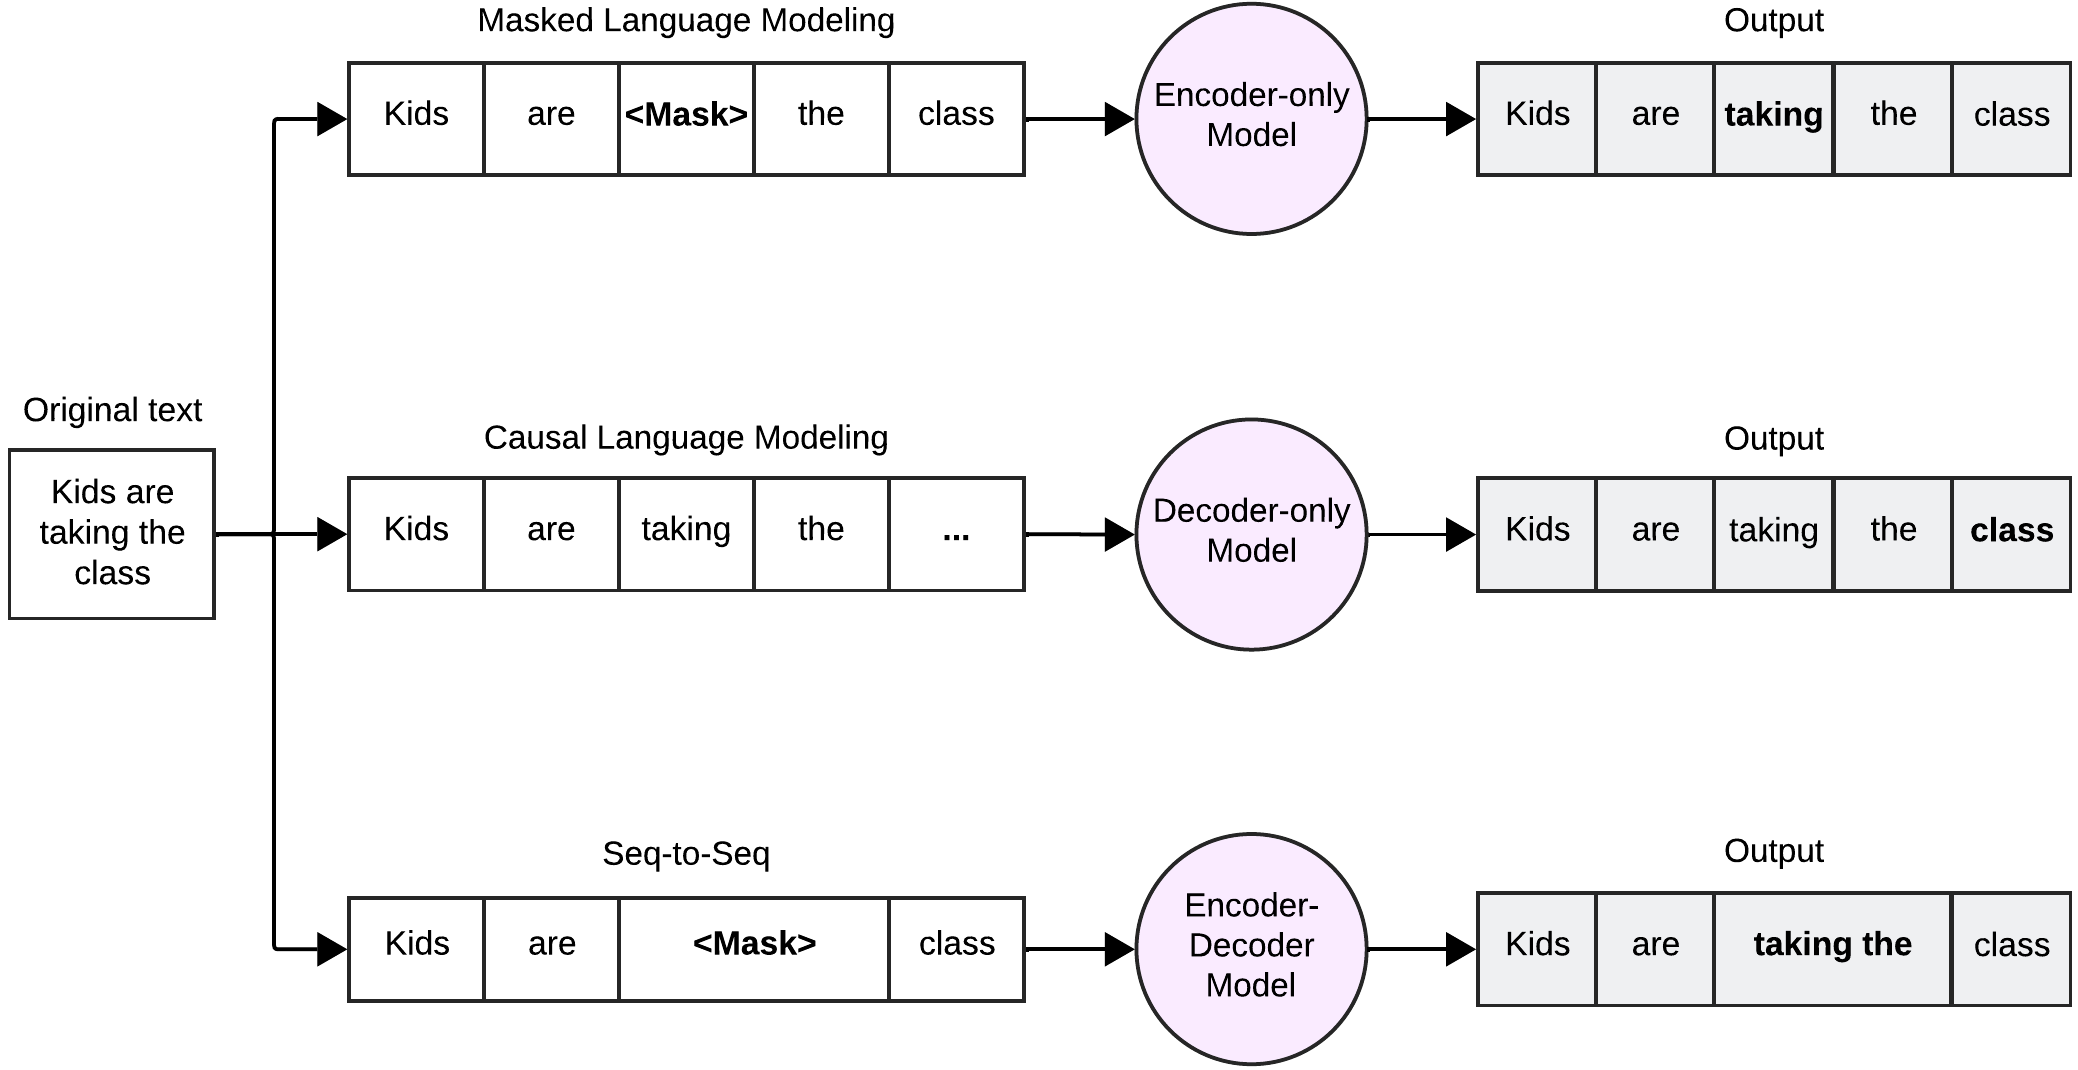
\includegraphics[width=\textwidth]{figures/LLM_Arch_text_generation.png}
        \caption{The transformer architecture}
        \label{architecture}
\end{figure*}

\subsection{Health Misinformation}
